\section{Primera revisión de los datos}\label{sec:exploracion}
Antes de construir un modelo revisamos los datos con cálculos sencillos. Lo que sigue son observaciones
preliminares. Antes de usarlas para decidir algo, alguien que no las haya calculado debe reproducirlas desde los
archivos originales (Tabla~\ref{tab:verificar}).

\subsection{Dos formas de registrar el rendimiento}
La Fig.~\ref{fig:regimenes} muestra el rendimiento de cada parcela por municipio. En cuatro municipios los valores
tienen dos decimales, como 4.47 o 4.52, y rondan 4.5~t/ha. En los otros cinco están redondeados a escalones de media
tonelada, como 2.5, 3.0 o 3.5, y rondan 3~t/ha. Por los decimales no sabemos si el rendimiento se midió de forma distinta, solo que se registró distinto. Llamamos \emph{régimen A} al primer grupo y \emph{régimen B} al
segundo (Tabla~\ref{tab:regimenes}).

\begin{figure*}[!t]
\centering
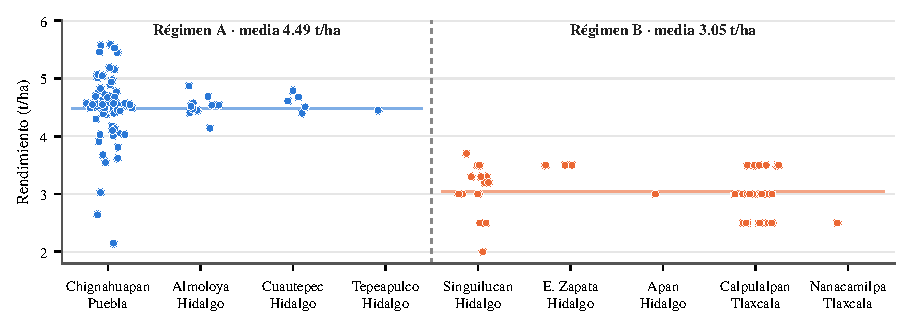
\includegraphics[width=\textwidth]{fig_regimenes}
\caption{Rendimiento de las 138 parcelas de entrenamiento por municipio. El color indica el régimen. En el régimen B
los valores se apilan en escalones de media tonelada.}\label{fig:regimenes}
\end{figure*}

\begin{table}[!t]
\caption{Rendimiento de entrenamiento por régimen}\label{tab:regimenes}
\centering\footnotesize
\begin{tabularx}{\columnwidth}{@{}lXrr@{}}
\toprule
Rég. & Municipios & Parcelas & Media (t/ha) \\
\midrule
A & Chignahuapan, Almoloya, Cuautepec de Hinojosa, Tepeapulco & 87 & 4.49 \\
B & Singuilucan, Emiliano Zapata, Apan, Calpulalpan, Nanacamilpa & 51 & 3.05 \\
\bottomrule
\end{tabularx}
\end{table}

\textbf{La separación no coincide con el estado.} El régimen se define por cómo está escrito el número, con decimales
o redondeado, y no por su valor. Hidalgo tiene municipios de los dos tipos. Almoloya, Cuautepec de Hinojosa y
Tepeapulco se parecen a Puebla, y Singuilucan, Emiliano Zapata y Apan se parecen a Tlaxcala. Agrupar por estado
mezcla dos poblaciones dentro de Hidalgo. El municipio también se conoce para las 59 parcelas de predicción, así que
el régimen se puede usar como variable.

\textbf{La causa todavía no es clara.} La diferencia puede ser real o puede deberse a la forma de registrar. Como la fuente del rendimiento es mixta, comercializadora y productor~\cite{preguntas}, una posible explicación, que no hemos confirmado, es que el redondeo dependa de quién reportó el dato en cada municipio. FIRA no entregará la fuente por parcela, así que no podremos comprobarlo. La estadística oficial de 2025 (SIAP) no compara lo mismo que las parcelas, porque es un promedio municipal de toda la superficie y no el rendimiento de parcelas puntuales. Aun así, la comparación deja dos observaciones. Considerando los nueve municipios, de los cuales la Tabla~\ref{tab:siap} muestra cinco, las etiquetas del reto superan al SIAP en 7, con 1.1~t/ha más en promedio, y el SIAP apenas separa los regímenes (3.0 contra 3.2~t/ha, ponderado por parcelas, frente a 4.49 contra 3.05 en las etiquetas). La correlación de rangos entre ambas series es de $-0.30$ con los cinco municipios de la tabla, y con $n=5$ no es concluyente. Además, Calpulalpan y Nanacamilpa tienen exactamente 4.00 en 2025 y entre 2.4 y 2.6 en 2023 y 2024, lo que podría indicar una cifra repetida para varios municipios. Por tanto, el SIAP sirve de contexto y no de validación. Por otro lado, las curvas de verdor sugieren que en el régimen B el ciclo es más corto, lo que podría
reflejar otra variedad o fecha de siembra. Para predecir, la causa importa poco, porque las 59 parcelas se califican
con etiquetas registradas, probablemente, igual que las de su municipio. Para interpretar los resultados sí importa, y conviene
preguntarlo a los organizadores.

\begin{table}[!t]
\caption{Media del reto y rendimiento municipal oficial de 2025, cebada de temporal~\cite{siap2026}}\label{tab:siap}
\centering\footnotesize
\begin{tabular}{@{}llrr@{}}
\toprule
Municipio & Rég. & Reto & SIAP 2025 \\
\midrule
Chignahuapan & A & 4.48 & 3.22 \\
Almoloya & A & 4.52 & 1.91 \\
Cuautepec de Hinojosa & A & 4.60 & 2.35 \\
Calpulalpan & B & 3.00 & 4.00 \\
Singuilucan & B & 3.08 & 1.88 \\
\bottomrule
\end{tabular}
\end{table}

\subsection{Valores extremos en parcelas pequeñas}
De los cinco rendimientos más altos (5.45 a 5.59~t/ha), cuatro son de parcelas de menos de 1.5 hectáreas
(Fig.~\ref{fig:area}), que son el 12\% de las parcelas de entrenamiento. Las cinco están en Chignahuapan. En general las parcelas más pequeñas rinden más, con una correlación de rangos de $-0.25$ con el área. Con mediciones de campo se ha documentado que los productores sobreestiman el rendimiento
sobre todo en parcelas pequeñas~\cite{gourlay2019,lobell2020}. Aquí una parte de los registros también viene del productor~\cite{preguntas}, así que parte de esos valores podría ser ruido de etiqueta. También podrían ser reales, por ejemplo por más manejo e insumos por hectárea en parcelas pequeñas. Con estos datos no podemos distinguir ambas posibilidades. Las parcelas pequeñas no muestran mayor dispersión que las demás.

\begin{figure}[!t]
\centering
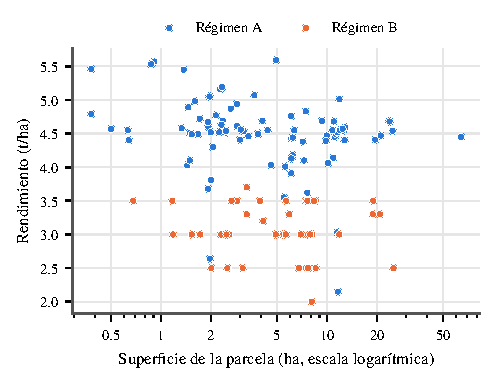
\includegraphics[width=\columnwidth]{fig_area}
\caption{Rendimiento frente al tamaño de la parcela, en escala logarítmica. Cuatro de los cinco rendimientos de
5.4~t/ha o más corresponden a parcelas de menos de 1.5 hectáreas.}\label{fig:area}
\end{figure}

\subsection{Error por redondeo}
Redondear a la media tonelada más cercana agrega un error típico de unas 0.14~t/ha, si el valor real
cae con igual probabilidad en cualquier punto del escalón. En el régimen B, 44 de las 51 etiquetas de entrenamiento son múltiplos de 0.5 y las otras 7 de 0.1. Con paso de 0.1 el error típico sería de 0.029~t/ha, y para la mezcla real del régimen B resulta 0.134~t/ha. Es una cota aproximada del orden de magnitud del error que un modelo perfecto no podría eliminar, no un piso exacto. El valor verdadero no tiene por qué ser uniforme dentro del escalón, y las etiquetas pueden tener otros errores mayores.

\subsection{La lluvia de 2025}
A nivel nacional, 2025 fue el año más lluvioso desde 1941. En la zona de las parcelas el total de mayo a octubre fue
parecido al de 2024 (951 contra 920~mm, frente a una normal de 679~mm), y lo que cambió fue el momento de la lluvia (Fig.~\ref{fig:lluvia} y Tabla~\ref{tab:lluvia}). La normal es el promedio de 2003 a 2024 de la misma fuente~\cite{funk2015}.
\begin{enumerate}
  \item \textbf{Mayo y junio fueron excepcionales}, con 384~mm, más del doble de lo normal (183~mm) y el máximo de 2003 a 2025. Eso favorece sembrar a tiempo, pero puede encharcar las parcelas recién sembradas.
  \item \textbf{Julio y agosto fueron normales} (281~mm contra 275~mm), sin exceso durante el llenado de grano.
  \item \textbf{Septiembre y octubre fueron altos pero no excepcionales}, con 286~mm, igual que en 2024 (287~mm) y 29\% sobre lo normal (221~mm). En esa etapa la lluvia
        puede tumbar el cultivo, lo que se conoce como \emph{acame}, o retrasar la cosecha.
  \item \textbf{La temperatura máxima fue más fresca} que en 2023 y 2024. Las temperaturas altas durante el llenado reducen el peso del grano~\cite{passarella2002}, así que una temperatura menor suele favorecerlo.
\end{enumerate}
Una posibilidad, que no hemos probado, es que los efectos del exceso de agua fueran de parcela, en zonas bajas o en parcelas sembradas o cosechadas tarde, y
no de zona. El clima mensual de 5 kilómetros difícilmente los detectaría.

\begin{figure}[!t]
\centering
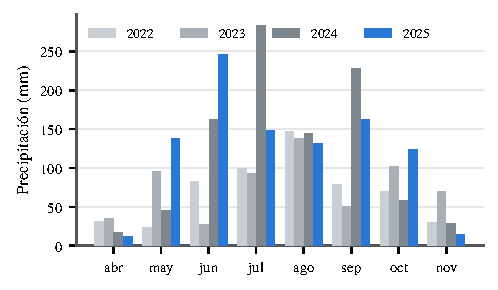
\includegraphics[width=\columnwidth]{fig_lluvia}
\caption{Precipitación mensual promedio sobre las 197 parcelas, de abril a noviembre~\cite{funk2015}.}\label{fig:lluvia}
\end{figure}

\begin{table}[!t]
\caption{Lluvia por etapa y temperatura máxima, promedio sobre las parcelas. La normal es el promedio de 2003 a 2024}\label{tab:lluvia}
\centering\footnotesize
\begin{tabular}{@{}lrrrrr@{}}
\toprule
 & 2022 & 2023 & 2024 & 2025 & Normal \\
\midrule
Mayo y junio (mm) & 106 & 122 & 207 & \textbf{384} & 183 \\
Julio y agosto (mm) & 246 & 231 & 427 & 281 & 275 \\
Septiembre y octubre (mm) & 148 & 154 & 287 & 286 & 221 \\
Tmax de mayo a sep. (°C) & 23.7 & 24.7 & 25.0 & 23.6 & - \\
\bottomrule
\end{tabular}
\end{table}

\subsection{Verificación}
La Tabla~\ref{tab:verificar} indica cómo comprobar cada observación. Distinguimos dos cosas. El dato es la cifra, y se confirma cuando otra persona reproduce el cálculo desde los archivos originales y obtiene los mismos números. La explicación de por qué ocurre es otra cosa y sigue sin probarse aunque el dato se confirme. Por ejemplo, que el redondeo dependa del municipio es un dato, y que se deba a la fuente del registro es una explicación pendiente.

\begin{table}[!t]
\caption{Observaciones preliminares y cómo comprobarlas}\label{tab:verificar}
\centering\footnotesize
\begin{tabularx}{\columnwidth}{@{}>{\raggedright\arraybackslash}p{3.3cm}X@{}}
\toprule
Observación & Cómo comprobarla \\
\midrule
Dos regímenes de registro por municipio & Contar por municipio los rendimientos con dos decimales y calcular la
  media de cada grupo \\
El régimen separa mejor que el estado & Comparar la varianza explicada por cada agrupación \\
Valores extremos en parcelas pequeñas & Graficar rendimiento contra área y revisar las cinco parcelas más altas \\
Lluvia de 2025 excepcional en mayo y junio & Extraer CHIRPS por parcela, sumar por bimestre y año y comparar con la normal \\
Más observaciones limpias en 2025 & Contar por año las fechas con nubosidad de 20\% o menos entre mayo y octubre \\
Planet cubre todo 2025 & Convertir las fechas con formato día, mes y año y revisar el rango \\
Ciclo más corto en el régimen B & Estimar inicio y fin del verdor por parcela y comparar entre regímenes \\
\bottomrule
\end{tabularx}
\end{table}
